% Cal Poly Thesis
%
% based on UC Thesis format
%
% modified by Mark Barry 2/07.
%


\documentclass[12pt]{ucthesis}

\usepackage{url}

\usepackage[pdftex]{graphicx}
\usepackage[pdftex,plainpages=false,breaklinks=true,colorlinks=true,urlcolor=blue,citecolor=blue,%
                                   linkcolor=blue,bookmarks=true,bookmarksopen=true,%
                                   bookmarksopenlevel=3,pdfstartview=FitV,
                                   pdfauthor={Marc Zych},
                                   pdftitle={An Analysis of Generational Caching Implemented in a Production Website},
                                   pdfkeywords={thesis, masters, cal poly}
                                   ]{hyperref}
%Options with pdfstartview are FitV, FitB and FitH
\pdfcompresslevel=1

\usepackage{amssymb}
\usepackage{amsmath}
\usepackage[letterpaper]{geometry}
\usepackage[overload]{textcase}
\usepackage{caption}
\usepackage{subcaption}
\usepackage{minted}

\bibliographystyle{abbrv}

\setlength{\parindent}{0.25in} \setlength{\parskip}{6pt}

\geometry{verbose,nohead,tmargin=1.25in,bmargin=1in,lmargin=1.5in,rmargin=1.3in}

\setcounter{tocdepth}{2}


% Different font in captions (single-spaced, bold) ------------
\newcommand{\captionfonts}{\small\bf\ssp}

\makeatletter  % Allow the use of @ in command names
\long\def\@makecaption#1#2{%
  \vskip\abovecaptionskip
  \sbox\@tempboxa{{\captionfonts #1: #2}}%
  \ifdim \wd\@tempboxa >\hsize
    {\captionfonts #1: #2\par}
  \else
    \hbox to\hsize{\hfil\box\@tempboxa\hfil}%
  \fi
  \vskip\belowcaptionskip}
\makeatother   % Cancel the effect of \makeatletter
% ---------------------------------------



\begin{document}

% Declarations for Front Matter

\title{An Analysis of Generational Caching Implemented in a Production Website}
\author{Marc Zych}
\degreemonth{June} \degreeyear{2013} \degree{Master of Science}
\defensemonth{June} \defenseyear{2013}
\numberofmembers{3} \chair{Alexander Dekhtyar, Ph.D.} \othermemberA{Philip Nico, Ph.D.} \othermemberB{Chris Lupo, Ph.D.} \field{Computer Science} \campus{San Luis Obispo}
\copyrightyears{seven}



\maketitle

\begin{frontmatter}

% Custom made for Cal Poly (by Mark Barry, modified by Andrew Tsui).
\copyrightpage

% Custom made for Cal Poly (by Andrew Tsui).
\committeemembershippage

\begin{abstract}
Web site scaling has been an issue since the inception of the web.
The demand for user generated content and personalized web pages leads to storing all content in a database on the web server.
Unfortunately, scaling the database to handle large amounts of traffic is still a problem many companies face.
One such company is \textsf{iFixit}, a provider of free, publicly-editable, online repair manuals.
Like many websites, \textsf{iFixit} uses \textsf{Memcached} to decrease database load and improve response time.
However, the caching strategy used is a very ad hoc one and therefore can be greatly improved.

Most research regarding web application caching focuses on cache invalidation, the process of keeping cached content consistent with the permanent data store.
Generational caching is a technique that involves including the object's last modified date in the cache key.
This ensures that cache keys change whenever the object is modified, which effectively invalidates all relevant cache entries.
Fine-grained caching is now very simple because the developer doesn't need to explicitly delete all possible cache keys that might need to be invalidated when an object is modified.
This is particularly useful for caching arbitrary fragments of HTML without increasing the complexity of cache invalidation.

We describe the process of implementing a caching strategy based on generational caching concepts in \textsf{iFixit}'s web site.
The results of our implementation show roughly X\% decrease in page response time and insert any other results here.
\end{abstract}


\tableofcontents


\listoftables

\listoffigures

\end{frontmatter}

\pagestyle{plain}




\renewcommand{\baselinestretch}{1.66}


\chapter{Introduction} \label{introduction}
Web scalability has been an issue for web sites since the dot-com boom of the late nineties \cite{webServerScaling}.
All moderately sized websites experience web server issues as their breadth of content as well as the number of active users grow.
If not properly addressed, the website's performance suffers.
In some cases the site can get overloaded by requests and stop responding altogether.
Websites need to be able to scale with their site traffic to continue providing a good user experience.

Some parts of website scaling are very straightforward.
Serving static assets such as Cascading Style Sheets (CSS), JavaScript (JS), and images can be offloaded to Content Delivery Networks (CDN) that handle requests separately from other resources such as the page's HTML.
Scaling application machines can be accomplished by sending all incoming requests to a load balancer.
The load balancer then decides what application machine in the cluster of available machines should handle this request.
The request is forwarded to the selected machine which eventually returns the HTML of the page to the load balancer which then returns it to the user.
Although application machines can be scaled easily, they all still need to access the same underlying data which is typically a single database machine.
The database is the hardest resource to scale because of the inherent problems in distributing data while maintaining consistency.

The ubiquitous solution to scaling websites is some form of caching.
Although most web servers employ generous amounts of caching, the methods and approaches used vary widely.
Client side browser caching is popular because it avoids a large amount of network overhead.
This is typically done by the server checking {\tt E-Tag} and/or {\tt Last-Modified} headers sent by the web browser to determine whether or not the content has changed since the client's previous request.
Proxy caching is very similar to browser caching except that it happens at proxy servers located in between the client and the primary host server.
This thesis, however, focuses on caching strategies and techniques in web application code that are aimed to reduce database load and decrease page response time.

Although application caching is used widely in industry, it is not a solved problem.
Websites still struggle with determining what data to cache and how fine-grained to make the cache entries.
Additionally, cache invalidation is the most important aspect of caching strategies and commonly is the driving force behind new solutions.
This is primarily because websites are becoming less tolerant of serving stale data especially when their content is constantly changing.
Current research is focused on maintaining a high cache hit rate while maintaining cache coherency.

Modern websites are interested in caching as a way to reduce response times and handle increasing volumes of traffic.
Traditional website scaling techniques aren't effective because of the vast amounts of user-generated content and dynamic nature of websites.
Nearly all web pages need to be generated on demand from content out of the database.
Because of this, server load becomes a real issue especially for the database machine.

\begin{figure}[h]
\centering
\includegraphics[width=\textwidth]{assets/iFixitHomepage.png}
\caption{iFixit's home page}
\label{fig:iFixitHomePage}
\end{figure}

One such website currently facing server scaling problems is \textsf{www.iFixit.com}, a moderately sized website that is ``the free repair manual that you can edit''\cite{ifixitDotCom} (Figure \ref{fig:iFixitHomePage}).
\textsf{iFixit}'s step-by-step guides and question-and-answer platform are driven largely by user-generated content.
All repair guides on \textsf{iFixit} are publicly editable and contain rich revision history.
Consequently, all of the content is stored in a database that must be queried in order to respond to requests for data.
To reduce server load and decrease response time, \textsf{iFixit} uses \textsf{Memcached}, an open-source in-memory caching system \cite{memcachedDotOrg}, to cache the results of expensive operations.
However, since the caching strategy used is an ad hoc one, the effectiveness of the cache can be greatly improved by using a different caching technique.

This thesis investigates web application caching techniques in the context of \textsf{iFixit}.
We focus on reducing page response time and server load by caching the results of database queries and HTML rendering.

Our work makes the following contributions:

\begin{enumerate}
   \item A survey of existing caching solutions applicable to web applications
   \item An in-depth description of implementing an adapted caching solution in \textsf{iFixit}'s code base
   % TODO: Specify generational caching here? And maybe provide background on what it is before this?
   % TODO: Include this? -- \item Provide a better understanding of when different caching strategies apply to certain situations, types of data, and access patterns.
   \item A performance comparison and analysis of experiments using real-world traffic
\end{enumerate}

The rest of this thesis is organized as follows.
Chapter \ref{background} provides background on caching and outlines related work, chapter \ref{designAndImplementation} describes the design and implementation of the caching system implemented in \textsf{iFixit}'s code base, chapter \ref{validation} validates our work, and chapter \ref{conclusions} concludes.


\chapter{Background} \label{background}
\section{Terminology}
At a high level, a cache is used to store results of operations so future requests can be processed faster.
A cache is typically not the primary storage location for data.
In most cases there is a permanent backing store such as a database which is used to retrieve information and populate the cache.
A cache entry is a single piece of data stored in the cache that can be uniquely identified.
A cache hit occurs when the requested cache entry is in the cache and no further action is required.
A cache miss occurs when the requested cache entry is not in the cache and it must be retrieved from its primary location.

Caching is effective because cache lookups are much faster than retrieving data from its persistent location.
Additionally, caching exploits locality.
Temporal locality is the idea that an item that has been referenced recently will likely be referenced again in the future.
Spatial locality is the idea that items in nearby storage locations are referenced in close proximity to one another.
As of late, spatial locality has been broadened for web sites to include access patterns such as recommended and related content.

Caches can be of the static or dynamic type.
A static cache is one that is not updated as a result of the application running.
The application can request data from the cache but it cannot add, modify, or remove cache entries.
However, the cache is periodically updated outside of the application to keep it mostly up to date.
The timeframe for this differs from application to application but is largely a function of how often the underlying data changes.
In contrast, a dynamic cache is one that can be updated as a result of the application execution.
The application can freely add, modify, and remove cache entries based on the operations it is performing due to requests.

Dynamic caches have a limited size and may eventually fill to capacity.
When this occurs items must be removed to make room for new ones.
The eviction policy determines which cache entries are removed.
A common eviction policy is Least Recently Used (LRU) which evicts the cache entry that has been accessed least recently.
Additionally, some caches allow entries to be set with an expire time.
After the specified time has passed, the entry is expired and future requests for it will result in a cache miss.

Cache coherence, also referred to as cache consistency, is the concept of keeping the data in the cache consistent with the data in the primary backing store.
One such method is to perform cache invalidation upon data modification which removes any modified items from the cache so the data must be generated upon the next request.
A cache stampede can occur when a cache that is frequently requested is invalidated.
There are then a series of cache misses followed by a series of duplicated requests to the backing store followed by a series of cache sets.
These should be avoided if possible because of the redundant work done by each request.
If not handled properly, a single cache stampede can crash web sites.

Database tables can specify a primary key which declares which columns of the table must have unique values for all tuples stored in the table.
Primary keys are useful for uniquely identifying tuples because {\tt SELECT} queries for explicit values of the primary key return at most one record.

The ActiveRecord pattern is a common technique used in web applications to interact with the data stored in a database.
In the host language, the developer creates classes that represent tables in the database.
This becomes an object-relational mapping (ORM) in that the properties of the class represent columns in the database.
Rows can be inserted, updated, and removed by calling the {\tt insert}, {\tt update}, {\tt delete} methods on the object, respectively.
This is demonstrated in Figure \ref{fig:activeRecordExample}.

\begin{figure}[h]
\begin{ssp}
\begin{minted}{php}
<?php
function createUser($userid, $name, $email) {
   $user = new User();
   $user->userid = $userid;
   $user->name = $name;
   $user->email = $email;
   $user->insert();
   return $user;
}

function getUser($userid) {
   $user = User::find($userid);
   return $user;
}
?>
\end{minted}
\end{ssp}
\caption{Basic ActiveRecord example.}
\label{fig:activeRecordExample}
\end{figure}

In this example, {\tt User} is a class that implements the ActiveRecord pattern.
A new user is inserted into the database by creating a new {\tt User} object, assigning the properties of the object corresponding to the database columns, and calling {\tt insert}.
This {\tt User} can later be retrieved by calling {\tt find}.


\section{iFixit}

\subsection{Data and Site Usage}
\textsf{iFixit}'s most popular content is their step-by-step repair guides, an example of which can be seen in Figure \ref{fig:iFixitGuideExample}.
An \textsf{iFixit} guide consists of an ordered list of steps as well as meta data about the guide such as title, summary, parts, and tools.
Each step consists of a list of bullet points with text, indentation, and color as well some sort of media such as a list of images or a video.
To avoid duplicating content, guides can also be included in other guides as prerequisites.
The guide is displayed to the user with its prerequisite guides' steps before the primary guide's steps.

\begin{figure}[hbtp]
\centering
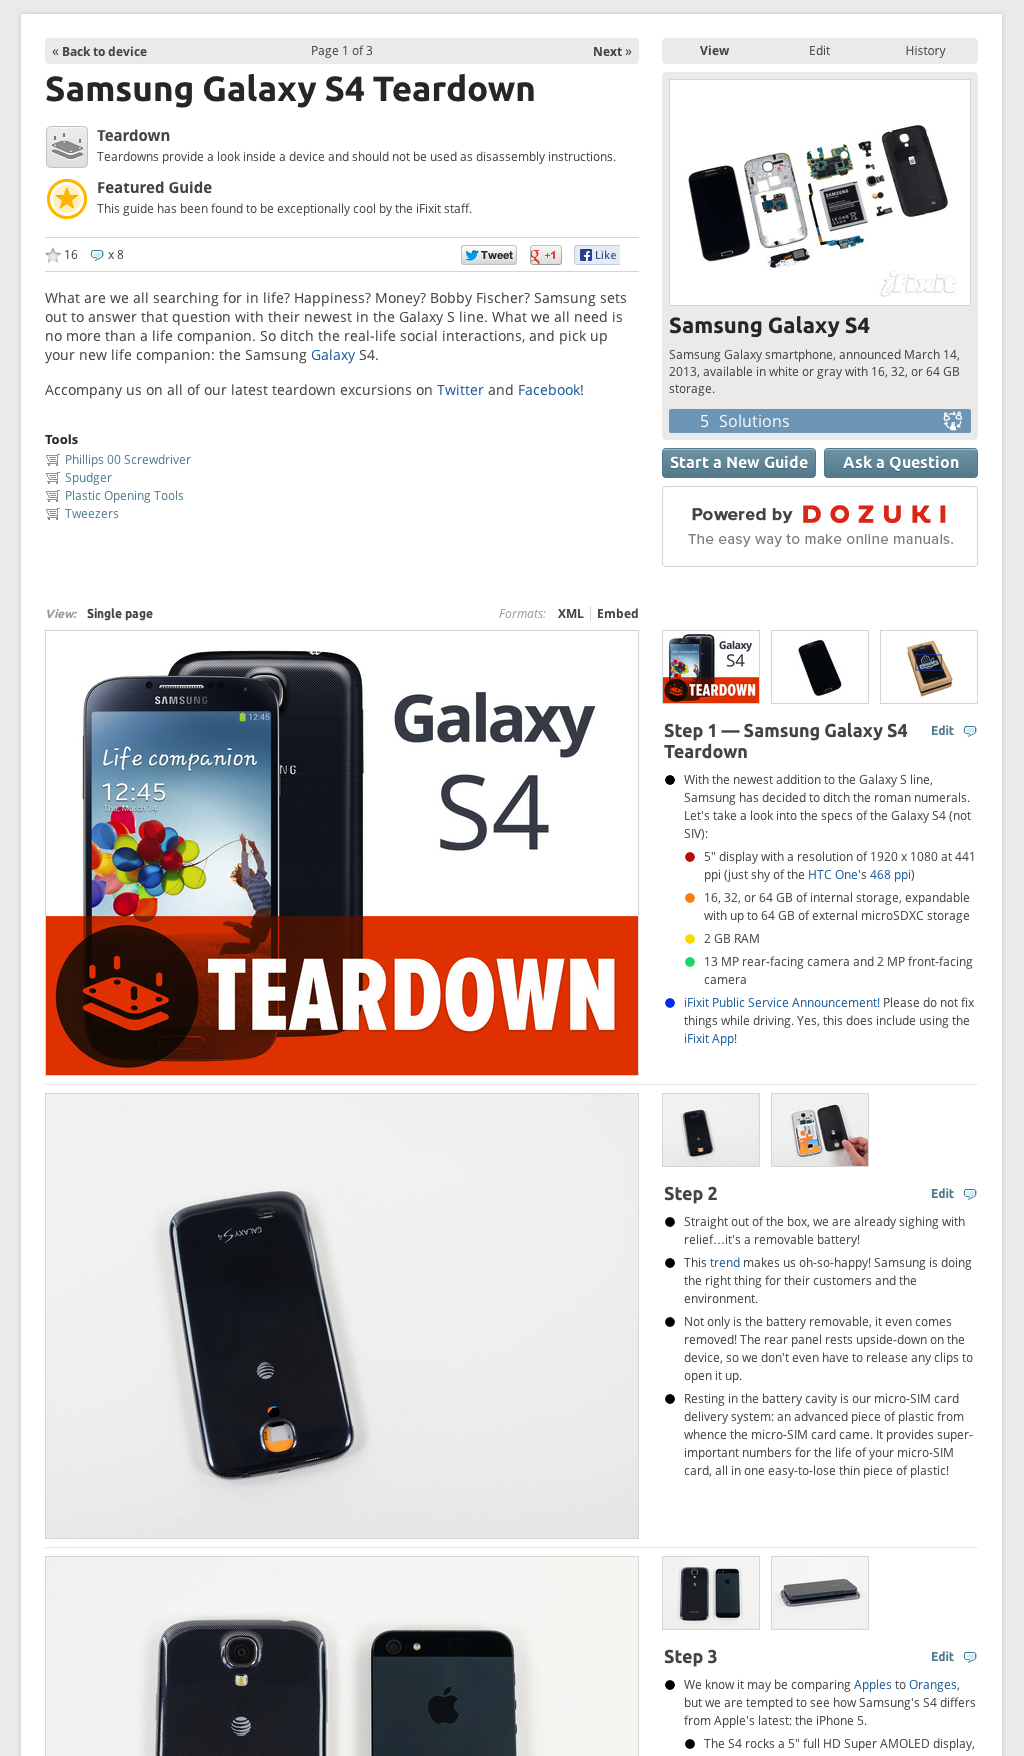
\includegraphics[width=\textwidth,height=0.95\textheight]{assets/iFixitGuideExample.png}
\caption{Example iFixit guide}
\label{fig:iFixitGuideExample}
\end{figure}

All of \textsf{iFixit}'s content is dynamic which means that handling requests involves gathering data from a database, rendering the page in the application language, and finally returning the resulting HTML to the user.
A dynamic website allows users to have rich, modifiable content that is always up-to-date.

\textsf{iFixit} certainly has a more read-heavy workload, however, writes are still fairly common.
Most notably, \textsf{iFixit} is known for its device ``teardowns.''
These events consist of opening a brand new device as soon as it becomes available on the market.
The opening process is documented and updated on \textsf{iFixit}'s website in realtime.
These events attract thousands of visitors to the site in a short period of time.
Because of this, the website must be able to handle a read-heavy workload while simultaneously writing to the same data.

In addition to their main website, \textsf{iFixit} runs \textsf{Dozuki}, a Software as a Service (SaaS) business that provides technical documentation to anyone who needs step-by-step instructions.
The same code base powers both \textsf{iFixit} and \textsf{Dozuki} which means that we are only interested in performance improvements to both platforms.
In particular, the general solutions to web scaling, such as full page caching and web server proxy caching, cannot be used because much of this content is private.

The primary bottleneck is the database machine because it has to retrieve data for every incoming HTTP request.
In contrast, application machines can easily scale horizontally by load balancing requests between them because they are stateless and operate independently of one another.
Sharding the data between multiple database machines to distribute the load is a common solution.
However, consistency and race conditions become major issues that must be addressed.

\subsection{Web Architecture}
In this section we describe \textsf{iFixit}'s production architecture, depicted in Figure \ref{fig:iFixitArchitecture}, at the time of this writing.
All of \textsf{iFixit}'s traffic goes directly to a load balancer which selects an application machine to handle the request.
At any given time there are four to eight application machines that run \textsf{iFixit}'s core software which is written in PHP.
They get all of their data from one master database machine running the Percona build of \textsf{MySQL} which handles all reads and writes.
There is also one slave database machine that is asynchronously replicated from the master database using \textsf{MySQL}'s built in replication.
However, this machine is used purely as a backup and is not used to improve performance.

All of this is built using Amazon Web Services (AWS) including Elastic Cloud Compute (EC2) for server instances, S3 for storing static assets and images, CloudFront, a Content Delivery Network (CDN), for serving content out of S3, and Elastic Block Store (EBS) for raw block storage on each server instance.

\begin{figure}[h]
\centering
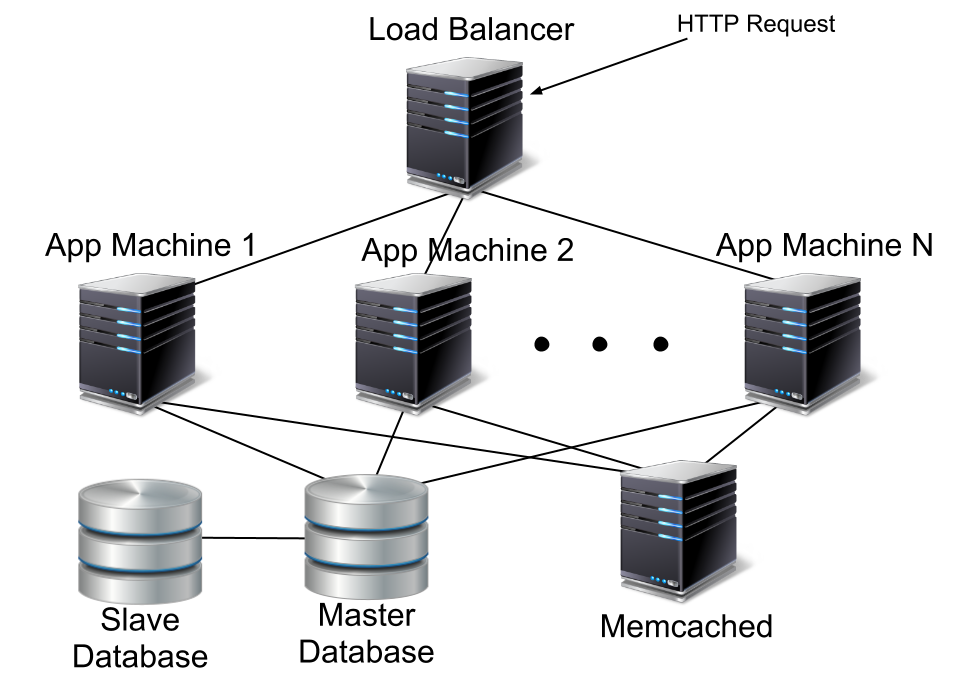
\includegraphics[width=\textwidth]{assets/iFixitArchitecture.png}
\caption{iFixit's Production Architecture}
\label{fig:iFixitArchitecture}
\end{figure}


\subsection{iFixit's Current Caching Strategy}
\textsf{iFixit} currently has a very ad hoc approach to caching.
Any specific pages, database queries, or expensive operations are guarded by a cache {\tt get} with a handcrafted cache key.
If the object is not in the cache, it is retrieved from the database and stored in the cache for later use.
The expiration time is typically on the order of minutes to hours depending on the method of invalidation for the data in question.
\textsf{iFixit} uses two strategies for cache invalidation that are described below.

The first strategy relies on the cache entry's expiration time to update it with fresh data.
After the specified amount of time, the cache is no longer valid so the application is forced to regenerate it and set it in the cache for later use.
The cache is never invalidated by the application when the underlying content changes.
This strategy is particularly useful for data that isn't required to be absolutely current such as related content, approximate totals, etc.

The second strategy used by \textsf{iFixit} involves deleting cache entries whenever relevant data is changed.
It is up to the developer to find the appropriate places to delete cache entries when certain events occur.
The advantages to this approach are that it's simple to understand, straightforward to implement, and ensures that fresh data is served if done correctly.

There are two major problems with these techniques.
The first is that the burden of cache invalidation is on the developer.
This is because the developer must decide what data to cache and spend time finding all the places where the cache entries should be invalidated.
Additionally, this is error-prone because software projects are constantly changing and the fragile caching setup could break.

The next problem is that caching HTML is difficult because each cache entry must be invalidated when data changes.
The more cache entries that depend on data, the harder it is to ensure that they will all be invalidated at the appropriate time.
This is especially true for fragments of HTML because the cache entries are typically defined in front-end templates but must be invalidated from back-end code.
In general, the difficulty of cache invalidation for any given datum is proportional to the number of cache entries dependent on that datum and how fine-grained those cache entries are.
As a result, \textsf{iFixit} doesn't currently cache any HTML fragments.

Our caching strategy aims to solve these two problems by providing a means for caching HTML and making cache invalidation happen automatically when the underlying data has changed.

\section{Related Work}
\subsection{Research Challenges}
Most research is focused on addressing two core challenges of caching: cache coherency and ease of use.
In some cases, maintaining cache coherency is trivial because there is only one cache entry associated with the underlying data.
However, with more complex data the situation is much more difficult.
There may be dependencies between objects which means that multiple cache entries need to be invalidated at the same time.
To further complicate things, the dependencies between objects may be dynamic and must be resolved at run time on a per object basis.
This is very common for Web 2.0 sites that are driven by user-generated content.

The second core caching challenge is ease-of-use.
The problem is that manually controlling the cache is tedious and error-prone.
Leaving it up to the application developer to correctly {\tt get}, {\tt set}, and {\tt delete} cache entries results in an ad hoc caching strategy.
Most research regarding ease-of-use focuses on developing a system that transparently handles all caching operations.
This leaves the developer to write application-specific code instead of caching boilerplate.

\subsection{Incorporating Cache}
\subsubsection{Caching Technologies}
Most web application caching research revolves around caching strategies.
It turns out that the underlying cache daemon is largely irrelevant.
\textsf{Memcached} is an example of a dynamic cache daemon which is well-suited for dynamic websites.
It is by far the most popular web caching system; it is currently in use by \textsf{Facebook}, \textsf{Wikipedia}, \textsf{YouTube}, and countless others \cite{memcachedDotOrg}.

Search engines use static caches as well because a large number of search queries return the same data for long periods of time.
These queries can be determined by analyzing historical data which would be difficult to do using a dynamic cache \cite{designTradeOffsSearchEngine}.
In particular, the knapsack problem can be used to fill the static cache if the request frequency and size of cacheable items can be determined \cite{designTradeOffsSearchEngine}.
Additionally, many papers propose a 2 or 3-level cache that incorporates both static and dynamic caches \cite{cacheAdmissionPolicies, designTradeOffsSearchEngine}.

The exception to this trend is Voras and Zagar's \textsf{Memcached} alternative, SQLCached \cite{sqlCached}.
This tool offers a few things that \textsf{Memcached} doesn't: complex data types and rich querying for retrieval and invalidation.
This is possible because SQLCached uses SQLite as its caching mechanism.

\subsubsection{Implementing in an Application}
Many approaches have been proposed for how to implement caching strategies in web application code.
The most straightforward method is to explicitly get, set, and invalidate caches wherever they are needed in the application.
However, this is tedious and error-prone \cite{keyBasedCacheExpiration, triggerBasedORM}.
A preferable alternative is to have caching built directly into the underlying application code.
For example, Ruby on Rails, a popular web framework, provides a very rich data model that handles most of the caching details behind the scenes \cite{keyBasedCacheExpiration}.

Gupta, Zeldovich, and Madden developed Cache Genie, an ORM for the Django web framework that automatically handles all necessary caching operations \cite{triggerBasedORM}.
The project registers Python callbacks for database triggers that are called when queries are run on the database.
This allows the tool to update and/or invalidate cache entries depending on the queries.
The major advantage of this approach is that no matter how the data is changed, the cache remains consistent because cache invalidation occurs at the data layer.
Other projects have used database triggers with similar results \cite{scalableConsistentCaching}.

\subsection{Cache Consistency}
\subsubsection{Write-Through Caching}
Write-through caching is a technique that involves saving the data in the cache at the same time as it is being saved in the persistent store \cite{writeThroughCaching}.
This technique improves cache hit rate because cache misses will only happen as a result of cache entry eviction or server failure.
However, this technique only works for simple data types.
Any other objects that depend on the current object being saved can't be updated in the cache because that data isn't directly accessible and will require a database lookup.

\subsubsection{Generational Caching}
Another caching technique is referred to as key-based cache expiration \cite{keyBasedCacheExpiration} and generational caching \cite{generationalCaching}.
The idea is that a timestamp, which corresponds to the last time the object was updated, is included in the key for any cache entries that depend on it.
The timestamp is updated every time the object is modified thus invalidating all necessary cache entries.
This approach also updates the timestamps of any objects that depend on the modified object.
Generational caching makes fine-grained caching trivial because it isn't necessary to enumerate all potential cache keys that depend on an object when it is modified.
Cache entries can be defined arbitrarily and as long as the cache key contains the timestamp it will be invalidated when the underlying object is updated.
This technique is employed by \textsf{37Signals}, a SaaS that provides project management tools and origin of the popular web application framework Ruby on Rails\cite{37SignalsDotCom}, and various other websites \cite{keyBasedCacheExpiration}.

One downside to this method is the amount of cache garbage that is generated because cache entries are never deleted.
However, this isn't much of an issue because most caching technologies use an LRU eviction policy so unused cache entries are eventually deleted when the cache fills up.
This is true of \textsf{Memcached} which is used by \textsf{37Signals} and \textsf{iFixit}.
Additionally, increasing the cache's capacity to make this even less of an issue is trivial with \textsf{Memcached}.

\subsubsection{Prefetching}
Prefetching content is another common solution for caching.
This technique involves caching content before it is requested so it can be retrieved quickly when it is needed.
Generally, an event triggers the precaching system to intelligently decide what content to prefetch in the hopes that the data will be requested soon.
This approach takes advantage of spatial locality.

Challenger, Iyengar, and Dantzig developed a caching system that addresses the problem of cache stampedes \cite{scalableConsistentCaching}.
Rather than invalidating any necessary cache entries when data changes, the fresh content can be prefetched and the cache's value will be updated in place using write-through caching.
This approach avoids cache misses at the cost of slight data staleness because the old copy will still be served while the fresh copy is being prefetched.
The website for the 1998 Winter Olympic games deployed this caching technique and reached nearly 100\% cache hits \cite{scalableConsistentCaching}.
Their system uses a dependency graph to determine which cache entries need to be updated when any given data is modified \cite{scalableConsistentCaching}.
When an object is updated, all of the cache entries that have an edge with that object need to be prefetched along with the original object.

Cambazoglu, Junqueira, and Plachouras use the cache expiration time to invalidate cache entries \cite{refreshingPerspectiveSearch}.
The idea is that serving slightly stale data isn't terrible for search engines.
Additionally, the rate of change can be determined for a given query and can be factored into the expiration time.
This allows frequently changing data to have a shorter time to live and infrequently changing data to have a longer time to live.

\subsection{Determining what to cache}
Some research has been done trying to determine what data is the most useful to cache.
Many sources propose that fragments of HTML are most useful because a cache hit for HTML allows the server to avoid generating the HTML as well as retrieving the underlying data from the persistent store \cite{comparisonOfCachingSolutions, scalableConsistentCaching, howBasecampGotSoFast}.

Baeza-Yates et al. suggested that enforcing cache admission policies is a valuable way to improve hit ratio \cite{cacheAdmissionPolicies}.
The driving idea behind it is that there are many singleton queries (queries that are run only once) that pollute the cache because they are not used again.
Detecting such queries and leaving them out of the cache leaves more room for caching results of frequently accessed queries thus increasing cache hit ratio.
However, Cambazoglu, Junqueira, and Plachouras claim that the eviction policy doesn't have a significant impact on cache hit ratio because caches can easily be expanded to hold more entries and therefore evictions are rare \cite{refreshingPerspectiveSearch}.


\section{Memcached}
In the words of its creators, \begin{quotation}``Memcached is an in-memory key-value store for small chunks of arbitrary data (strings, objects) from results of database calls, API calls, or page rendering\cite{memcachedDotOrg}.''\end{quotation}
There are two main operations in \textsf{Memcached}: {\tt get} and {\tt set}.
Clients perform {\tt get} calls by passing in a string cache key that identifies the data that is being requested.
For example, {\tt users-1234} could be used to identify the {\tt User} object with {\tt userid} of {\tt 1234}.
The data is returned to the caller if it is in the cache, otherwise the application must retrieve the data from its primary location.
Data is added to \textsf{Memcached} by calling {\tt set} with a cache key, expiration time, and the data to store in the cache.
Another specialty command is {\tt getMulti} which is used to retrieve multiple keys in one operation.
This is used to improve client performance by reducing the network overhead associated with retrieving many keys in succession.
All \textsf{Memcached} operations are constant time ({\tt O(1)}) with respect to the number of elements stored in it.

There are three ways for cached data to be removed from \textsf{Memcached}.
The expire time the data was set with determines the maximum lifespan of the cache entry for which it is valid.
Once the data has expired it is no longer returned for {\tt get} requests although the data is not immediately removed from memory.
Before data has expired, however, items can be evicted due to memory pressure.
This occurs when new items are being added to the cache and there isn't any room.
Expired items are evicted first if any are found, otherwise the Least Recently Used (LRU) policy is used to select a cache entry to evict.
In other words, the cache entry that has last been referenced the longest ago is evicted.
Finally, cache entries can also be removed by performing {\tt delete} requests and providing the key that identifies the data to be deleted.

To reduce the effects of memory fragmentation, \textsf{Memcached} employs a technique called slab allocation.
The total memory available to \textsf{Memcached} is partitioned into 1MB pages.
Pages are assigned to slab-classes on an as-needed basis.
Slab-classes determine the maximum size of data to be stored in the slab and consequently the size of chunks in pages assigned to the slab-class.
When storing data in \textsf{Memcached}, the slab-class with the smallest chunk size that the data can fit in is used.
Any remaining space in the chunk cannot be used to store any other data and therefore ends up being wasted space.
However, the amount of space wasted in slab allocation is less than a naive implementation which results in memory fragmentation.
All replacement algorithms operate on a per-slab-class basis.

\textsf{Memcached} is distributed in nature.
Adding more servers to a web application involves adding the new \textsf{Memcached} instance's IP address and port to the list of servers that the \textsf{Memcached} client library uses.
Keys map to exactly one server so the total memory available in the \textsf{Memcached} cluster is the sum of memory available on each instance.
The client library performs consistent hashing\cite{consistentHashing} on any key lookups to determine which server in the cluster to send the request to.
The result is that adding and removing servers doesn't drastically impact hit rate because the majority of keys map to the same servers before and after the change.


\chapter{Design and Implementation} \label{designAndImplementation}
In this chapter, we explain in depth the caching solution we implemented for \textsf{iFixit} and analyze in Chapter X.
But first, we must reiterate \textsf{iFixit}'s requirements for such a caching solution.

\begin{description}
   \item[R1] The caching strategy must be largely transparent to the developer.
             The developer should only be required to determine what data to cache, not how to cache it and how to invalidate it.
   \item[R2] The caching strategy must allow for finer-grained caching without added complexity.
   \item[R3] The caching strategy must provide a means of caching and invalidating fragments of HTML.
   \item[R4] The caching strategy must result in increased performance in regards to response time and database load. % TODO: Not database load because it's hard to measure? Or it isn't since query count/exec time is good? Be more specific?
\end{description}

The rest of this chapter is organized as follows.
In section 3.1 we explain the high-level design of the caching strategy implemented for \textsf{iFixit}.
In section 3.2 we go over the details of implementing the design in \textsf{iFixit}'s code base.

\section{Design}
Out of existing solutions, generational caching most closely meets these requirements because the cache key changes whenever the underlying data changes, so cache entries no longer need to be explicitly invalidated.
This allows there to be many cache entries that depend on a single piece of data and the values will not need to be invalidated.
For these reasons, we used generational caching concepts as a starting point for our caching solution.

\subsection{What is being cached}
This section describes the three primary types of data that are cached in our caching strategy.
The first data type is objects constructed from query results that represent a tuple in the database (see Figure \ref{fig:ormObject}).
These are used as an ORM which can make modifications to the database as well as retrieve data for consumption.
The second data type is fragments of HTML generated in templates like the one depicted in Figure \ref{fig:htmlTemplate}.
These typically produce output based on data retrieved from the database and need to be invalidated anytime that data has changed.
Finally, results of ad hoc queries, like the one in Figure \ref{fig:adHocQuery}, are also cached.
These typically are used in addition to the ORM to gather more complex data.

\begin{figure}[hbtp]
\begin{subfigure}[b]{1.0\textwidth}
\begin{ssp}
\begin{minted}{php}
<?php
class Guide extends ORMObject {
   private $guideid;
   private $langid;
   private $title;
   private $difficulty;
   private $steps;
}
?>
\end{minted}
\end{ssp}
\caption{ORM Object}
\label{fig:ormObject}
\end{subfigure}

\begin{subfigure}[b]{1.0\textwidth}
\begin{ssp}
\begin{minted}{php}
<div class="guide">
   <h3><?= $guide->title ?></h3>
   <p>Difficulty: <?= $guide->difficulty ?></p>
   <div class="steps">
   <? foreach ($guide->steps as $step): ?>
      <div class="step">
         <?= $step->title ?>
      </div>
   <? endforeach ?>
   </div>
</div>
\end{minted}
\end{ssp}
\caption{HTML template}
\label{fig:htmlTemplate}
\end{subfigure}

\begin{subfigure}[b]{1.0\textwidth}
\begin{ssp}
\begin{minted}{sql}
SELECT guideid, langid
FROM guide_prereqs
WHERE prereq_guideid = ? AND prereq_langid = ?
\end{minted}
\end{ssp}
\caption{Ad hoc query}
\label{fig:adHocQuery}
\end{subfigure}

\caption{Data types being cached}
\label{fig:dataBeingCached}
\end{figure}

\subsection{Caching Approach}
We will first discuss how we incorporate caching into our ORM and how it is used for \textsf{iFixit}'s guides.
The guide and step ORM objects can be found in Figure \ref{fig:cachingExample}.

The primary key of a database table can be used with the ORM to select a single record.
Once the record is loaded, other data not contained in the primary table is loaded and then the entire object is cached.
For guides, the {\tt Guide} object is retrieved from the DB and then the {\tt Step} objects are loaded afterwards.
By default, the cache key for objects is just the values of primary key columns.

Generational caching relies on a value in the primary table being updated whenever any other data in the table is updated.
This value can be incorporated into the object's cache key which ensures that the value in the cache will always be correct for that cache key.
If the data changes then it has a different cache key so the other cache entries don't need to be invalidated.
To accomplish this, individual classes extending the ORM specify what columns in addition to the primary key to include in the cache key.
For guides, this value is the {\tt modified\_date} which is set to the current time in microseconds anytime the guide or any of its children are modified.
For example, a {\tt Guide} could have cache keys {\tt Guide/1234-en-1368160868.395738} and {\tt Guide/1234-en-1368173958.773968} before and after it is modified, respectively.

In most cases, the additional columns are not known before retrieving the object and must be retrieved before checking the cache.
This is typically because the request URL only specifies the primary key and not any other additional information.
To avoid hitting the database as much as possible, the entire database tuple that is used to generate the cache key is cached using its primary key.
This cache entry is deleted anytime the object is saved.

For example, only the {\tt guideid} and {\tt langid} are initially available when a guide request hits {\tt iFixit}'s servers.
For a {\tt guideid} of {\tt 1234} and {\tt langid} of {\tt en}, the cache is checked for the {\tt Guide} object using {\tt Guide/1234-en} as the cache key.
If it isn't found in the cache, it is retrieved from the database and stored in the cache.
This object does not contain any data from other tables such as {\tt Steps}.
The full cache key can then be constructed, for example {\tt Guide/1234-en-1368164354.918344}, and used to fetch the rest of the content.
If it exists in the cache then it can be returned to the caller immediately.
Otherwise, it must be retrieved from the database.
Fortunately, the primary table tuple has already been fetched from the database so we only need to load the additional data for the object and store it in the cache.

This strategy works especially well when retrieving an object's additional data is very expensive.
If no additional data is loaded then the ``fully loaded'' object is the exact same as the one fetched when gathering more data to construct the cache key.
In this case there is no benefit to using generational caching because the data cached by the primary key is the same as the data cached with the full set of columns.
However, the additional columns can be used in cache keys for data that depends on it to avoid cache invalidation.
The amount of extra data loaded in addition to the primary table to make the overhead of generational caching worthwhile varies on a case-by-case basis.
This approach is effective for {\tt Guide}s because there is a large amount of additional data to retrieve.
Although only {\tt Step}s are described in this example, there are several other tables that must be queried to display a guide to the user.

For fragments of HTML and ad hoc query results that can only change when the ORM object changes, the object's full cache key can be used in addition to a qualifying string such as {\tt view-all-html}.
Any cache entry that does this will be automatically invalidated when the object changes because the cache key will change.
This allows for fine-grained caching without the need to enumerate and delete all keys that depend on an object.

Occasionally HTML fragments contain data that changes at different times than the ORM object.
That value could be incorporated into the cache key but it would fragment the cache into many different possibilities thus reducing its effectiveness.
For example, {\tt Step}s' {\tt revisionids} are updated every time they are modified.
However, the step number displayed to the user can be different for the same step on different guides because of the order of prerequisite guides.
Rather than including the step number in the cache key, a placeholder value is used in place of the step number, which is replaced with the actual step number before it is output to the user.

\begin{figure}[h]
\begin{subfigure}[h]{0.5\textwidth}
\begin{ssp}
\begin{minted}{php}
<?php
class Guide extends ORMObject {
   protected static $cacheCols =
    ['modified_date'];

   // Primary key.
   protected $guideid;
   protected $langid;

   // Columns from guide table.
   protected $title;
   protected $difficulty;
   protected $modified_date;
   protected $revisionid;

   // Retrieved from other tables.
   protected $steps;
   protected $parts;
}
?>
\end{minted}
\end{ssp}
\caption{Guide ORM object}
\label{fig:guideORMTable}
\end{subfigure}
\begin{subfigure}[h]{0.5\textwidth}
\begin{ssp}
\begin{minted}{php}
<?php
class Step extends ORMObject {
   protected static $cacheCols =
    ['revisionid'];

   // Primary key.
   private $stepid;

   // Columns from step table.
   private $guideid;
   private $langid;
   private $title;
   private $orderby;
   private $revisionid;

   // Retrieved from other tables.
   private $media;
   private $lines;
}
?>
\end{minted}
\end{ssp}
\caption{Step ORM object}
\label{fig:stepORMObject}
\end{subfigure}
\caption{Example guide and step ORM objects}
\label{fig:cachingExample}
\end{figure}


\section{Implementation}
\subsection{Existing Infrastructure}
Before we can go into the details of the implementation of generational caching, some background on \textsf{iFixit}'s existing code must be presented.
Most data is retrieved using a custom ORM that was built in-house.
The primary operation for retrieving data through the ORM is {\tt findAllByKey} which returns objects based on their primary keys in the database.
A list of primary keys is provided to {\tt findAllByKey} and the ORM selects those tuples from the database and returns the objects constructed from them.

\subsection{Cache-Aware ORM}
Most of the work performed while implementing the caching strategy involved augmenting \textsf{iFixit}'s ORM to cache objects when they are retrieved with {\tt findAllByKey}.
In order to add caching to {\tt findAllByKey} we add a wrapper method called {\tt findAllCached}.
At a very high-level, this method constructs cache keys for the given primary keys and performs a cache {\tt getMulti} on them.
Any objects that were not cached are retrieved from the database using {\tt findAllByKey} and are then stored in the cache.

We allow classes derived from the ORM to specify which columns, in addition to the primary key, to include in the cache key.
More data must be retrieved from the database to construct the cache key if only the primary keys are provided to {\tt findAllCached} and the derived class specifies additional cache key columns.
Fortunately, we already have a method, {\tt findAllByKey}, that retrieves objects based on their primary key that can be used to retrieve more data.
However, we can do one better and cache that operation by using {\tt findAllCached} instead.
For this call, a flag is passed to {\tt findAllCached} that indicates that only the primary table should be loaded.
Otherwise, all other relevant data would be loaded which is exactly what the first {\tt findAllCached} call does.
The recursive call constructs a cache key using only the primary key to avoid infinite recursion.

The \textsf{Memcached} operations are performed using {\tt getMulti} to minimize the network overhead involved in doing multiple sequential \textsf{Memcached} {\tt get}s.
All cached objects are retrieved with one {\tt getMulti} call and the uncached objects are retrieved with one database query and are cached for later use.

\subsection{Caching HTML and Ad Hoc Queries}
We also cache fragments of HTML because HTML generation can be fairly slow and unperforming.
To help facilitate this, we implemented a few different caching functions for use in HTML templates.

The first set of functions is {\tt cacheStart} and {\tt cacheEnd} which are used for caching a single block of HTML.
{\tt cacheStart} accepts either an object that has a {\tt cacheKey} method (e.g. an ORM object) or a string cache key.
Another string is supplied that is added to the cache key to differentiate this fragment of HTML from other fragments constructed from the same object.
If the HTML was found in the cache it is output to {\tt stdout} and {\tt cacheStart} returns {\tt true}.
Otherwise output buffering is started to capture the HTML that is generated when running the template code and {\tt cacheStart} returns {\tt false}.
A call to {\tt cacheEnd} signals the end of the cached HTML section.
This function closes output buffering, gets the contents of the buffer, caches it, and finally outputs the HTML to {\tt stdout}.
A basic example is shown in Figure \ref{fig:cacheStartExample}.

\begin{figure}[h]
\begin{ssp}
\begin{minted}{php}
<? if (!cacheStart($guide, 'view-all', CACHE_FOREVER)): ?>
   <div class="guide">
      <h3><?= $guide->title ?></h3>
      <p>Difficulty: <?= $guide->difficulty ?></p>
      <? /* Step HTML generation. */ ?>
   </div>
<? cacheEnd(); endif ?>
\end{minted}
\end{ssp}
\caption{Example usage of cacheStart and cacheEnd}
\label{fig:cacheStartExample}
\end{figure}

\begin{figure}[hbtp]
\begin{ssp}
\begin{minted}{php}
<?php
function batchCache($cacheKeys, $where, $expire,
 $renderFunction) {
   $templateCacheKeys = [];
   foreach ($cacheKeys as $key => $id) {
      $templateCacheKeys["$key-$where"] = $id;
   }

   $allHtml = cacheGetMulti($templateCacheKeys, $expire,
      function($missing) use ($renderFunction) {
         $found = [];

         foreach ($missing as $cacheKey => $id) {
            ob_start(); {
               $renderFunction(array_shift($misses));
               $html = ob_get_contents();
            } ob_end_clean();

            $found[$cacheKey] = $html;
         }

         return $found;
      }
   );

   foreach ($allHtml as $html) {
      echo $html;
   }
}
?>
\end{minted}
\end{ssp}
\caption{Implementation of batchCache}
\label{fig:batchCacheImplementation}
\end{figure}

The second caching function we wrote is {\tt batchCache} which is designed for caching multiple fragments of HTML.
The most common use case for it is rendering a list of objects one after the other e.g. search results.
{\tt batchCache} is better than {\tt cacheStart} and {\tt cacheEnd} for this circumstance because of the network overhead for sequential \textsf{Memcached} calls.
This is especially true for fragments of HTML whose generation time is close to or less than the average time of a \textsf{Memcached} {\tt get}.
{\tt batchCache} minimizes network overhead by using \textsf{Memcached}'s {\tt getMulti} operation.

The implementation of {\tt batchCache} is depicted in Figure \ref{fig:batchCacheImplementation}.
{\tt batchCache} accepts an array of ORM objects and, much like {\tt cacheStart}, an additional string to differentiate these cache entries from others constructed from the same objects.
{\tt batchCache} calls \textsf{Memcached} {\tt getMulti} with the cache keys identifying the provided objects. % TODO: This is super vague.
For each cache miss, output buffering is started and the supplied rendering function is called with the ORM object.
Output buffering is then closed and the resulting HTML is stored in the cache and added to the array of resulting HTML. % TODO: Fix the awkwardness of this sentence.
Finally, every fragment of HTML is output to {\tt stdout} in the same order that their corresponding objects were provided.
This is demonstrated for {\tt Step}s in Figure \ref{fig:batchCacheStep}, which is the cached steps version of Figure \ref{fig:htmlTemplate}.

\begin{figure}[h]
\begin{ssp}
\begin{minted}{php}
<div class="steps">
<? batchCache($guide->steps, 'step_view', CACHE_FOREVER,
    function($step) { ?>
   <div class="step">
      <?= $step->title ?>
   </div>
<? }); ?>
</div>
\end{minted}
\end{ssp}
\caption{Example usage of batchCache for Steps}
\label{fig:batchCacheStep}
\end{figure}

The same approach can be applied to caching ad hoc query results.
Figure \ref{fig:adHocQueryCaching} demonstrates this by using {\tt cacheGetAndSet}.
The cache key is constructed using the guide's full cache key and the string {\tt -prereqs}, so it will be invalidated when the guide is modified.
If the value is not cached, {\tt cacheGetAndSet} calls the provided function and caches the result.

\begin{figure}[h]
\begin{ssp}
\begin{minted}{php}
<?php
$cacheKey = $guide->cacheKey() . "-prereqs";
$prereqs = cacheGetAndSet($cacheKey, function() use ($guide) {
   return dbQuery("
      SELECT guideid, langid
      FROM guide_prereqs
      WHERE prereq_guideid = ? AND prereq_langid = ?",
    [$guide->guideid, $guide->langid]);
});
?>
\end{minted}
\end{ssp}
\caption{Ad hoc query caching}
\label{fig:adHocQueryCaching}
\end{figure}


\chapter{Validation} \label{validation}
Validation is a fairly straightforward process.
The basic approach involves gathering various statistics with and without our caching strategy during an experiment based on a repeatable and representative set of input data.

\section{Experimental Setup}
We recorded requests to \textsf{www.iFixit.com} for a full week and selected two 24-hour sets of representative data to use as input to the experiments.
The first data set is typical traffic during a weekday which involves accessing a high breadth of content at a fairly steady pace.
The second data set is traffic during \textsf{iFixit}'s Samsung Galaxy S4 Teardown\cite{ifixitGalaxyS4Teardown}, which involves a large number of reads and writes to the same resource.

Since our caching strategy was only applied to guides, the request logs are filtered to only include requests viewing or modifying guides.
Otherwise, the results would be affected by other non-guide requests which are not using our generational caching method.

The test environment, depicted in Figure \ref{fig:experimentalArchitecture}, is an isolated clone of \textsf{iFixit}'s production architecture consisting of a load balancer, two application machines, and a database machine.
Since the traffic replays are a subset of \textsf{iFixit}'s traffic, two application machines are more than enough to handle the load.
All machines are AWS EC2 nodes running 64-bit CentOS 5.4.
The load balancer is a {\tt m1.large} instance with 7.5 GiB memory and 4 EC2 Compute Units (2 virtual cores with 2 EC2 Compute Units each).
This machine runs \textsf{Memcached} {\tt 1.4.15} which is used by the application machines.
The database machine is a {\tt m1.xlarge} instance with 15 GiB of memory and 8 EC2 Compute Units (4 virtual cores with 2 EC2 Compute Units each).
This machine runs \textsf{MySQL} {\tt 5.5.29 Percona Server} with EBS-striped volumes.
The application machines are {\tt c1.medium} instances with 1.7 GiB of memory and 5 EC2 Compute Units (2 virtual cores with 2.5 EC2 Compute Units each).
More information regarding EC2 specs can be found on AWS's website \cite{awsInstanceTypes}.

% TODo: Change HTTP request to be simulated requests coming from and to the load balancer.
\begin{figure}[h]
\centering
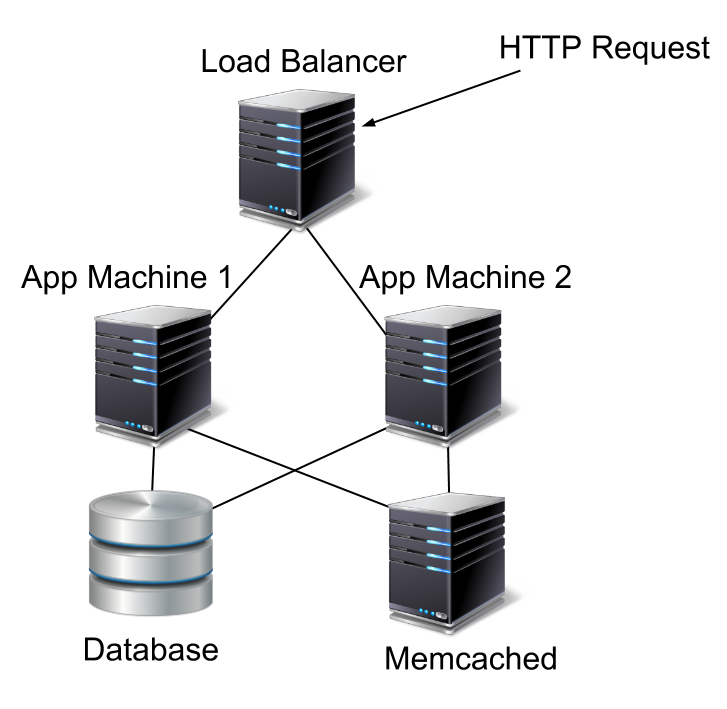
\includegraphics[width=\textwidth]{assets/experimentalArchitecture.png}
\caption{Experimental Setup}
\label{fig:experimentalArchitecture}
\end{figure}


We then replay the requests in the 2 test sets with and without our caching strategy for a total of 4 runs.
Requests are performed using a NodeJS script running on the load balancer making requests to {\tt localhost} to reduce latency between the simulated client and the web servers.
Every request is profiled server-side --- \textsf{Memcached}, \textsf{MySQL}, and CPU usage statistics are recorded to the database.

Before each experiment is run, the database is restored to the state it was in when the requests were originally made to \textsf{www.iFixit.com}.
This ensures that the data is the same between runs and all views and edits are working with the same data.
The stats logging table is truncated, so only requests during the experiment are in the table when the test is complete.
Finally, \textsf{Memcached} is restarted, which empties its contents.

The experiment is then run for the full 24 hours.
Afterwards, the stats logging table is extracted using {\tt mysqldump} so the data can later be analyzed.

\section{Measured Values}
The most general value we compare is \textit{page response time}, the total amount of time the request spent on our servers.
Response time should decrease because more data is cached and can be returned faster than before.
Similarly, \textit{HTML generation time} should decrease because fragments of HTML are now being cached.

The interesting values for \textsf{Memcached} stats are \textit{get count}, \textit{hit rate}, and \textit{time spent in cache calls}.
The get count will likely increase because cache entries are finer-grained.
Cache hit rate will vary drastically because pages with uncached content will have a large number of misses.
However, pages with cached content will have either a few cache hits for a large amount of content or many cache hits for finer-grained content.
In general, cache hit rate should increase because cache entries aren't set to expire and the only misses will be for new or changed content.
Time spent in \textsf{Memcached} calls will likely increase because more content is being cached.

Finally, the interesting values for \textsf{MySQL} are \textit{query count} and \textit{total query time}.
Query count should go down because the cache should serve more requests that previously were handled by the database.
Additionally, network overhead is reduuced because more content is retrieved in batch using fewer queries.
Both of these should cause a decrease in total database query time.

\section{Hypothesis}
% TODO: Write.

\section{Results}
% TODO: Write. Pretty much a raw data dump of stuff.

\section{Analysis}
% TODO: Analyze results. Draw conclusions. Explain stuff.


\chapter{Conclusions and Future Work} \label{conclusions}

% TODO: Write.

\section{Future Work Ideas}
How size of cache affects hit rate over long periods of time to evaluate if it's okay to not invalidate anything.


% ------------- End main chapters ----------------------

\clearpage
\bibliography{thesis}
\bibliographystyle{plain}
%\addcontentsline{toc}{chapter}{Bibliography}

\end{document}
